\section{Introduction}

Time series forecasting is pivotal for modern decision-making, enabling strategic resource allocation in critical sectors ranging from energy~\citep{zhou2021informer} and traffic~\citep{li2018dcrnn} to finance and weather~\citep{jin2024surveygnn}. Driven by this practical value, the field has rapidly evolved from traditional statistical methods to sophisticated deep learning paradigms~\citep{makridakis2018m4, wen2022transformers}. Consequently, developing robust models capable of generalizing across these diverse, dynamic scenarios remains a critical challenge in machine learning.
In pursuit of superior forecasting, current research primarily diverges into two paths. Specialized Transformer architectures, such as PatchTST~\citep{nie2022time} and iTransformer~\citep{liu2023itransformer}, effectively capture temporal dependencies but often lack the cross-domain transferability of foundation models. Consequently, recent works have adapted Large Language Models (LLMs)~\citep{zhou2023one, jin2024timellm} and Large Vision Models (LVMs)~\citep{shen2025dmmv, zhong2025time} for time series tasks. However, the prevailing ``Align-then-Tune'' paradigm, exemplified by Time-LLM~\citep{jin2024timellm}, treats time series as a foreign modality. This approach necessitates complex \textbf{pre-alignment} modules such as reprogramming layers to map continuous numerical tokens into the semantic space prior to fine-tuning.
However, "Align-then-Tune" strategies face two intrinsic limitations. First, a fundamental \textbf{granularity mismatch} persists between continuous high-dimensional time series and discrete linguistic space; forcing numerical fluctuations into embeddings inevitably causes \textit{information loss}, obscuring critical temporal dynamics during the translation process. Second, reliance on explicit pre-alignment creates significant \textbf{architectural overhead}. These auxiliary modules act as bottlenecks, effectively preventing the LLM from directly applying its inherent reasoning capabilities to the raw numerical data.

\begin{figure}[htbp]
  \centering

  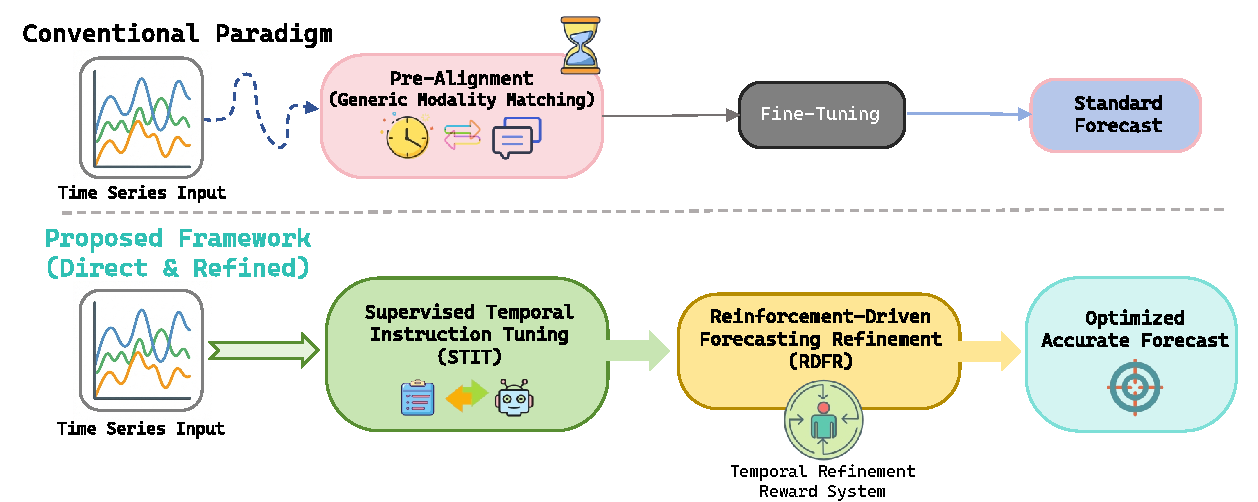
\includegraphics[width=0.75\linewidth]{figures/Intro.pdf}

  \caption{Comparison of forecasting paradigms. Conventional approaches~\cite{zhou2023one,jin2024timellm} rely on pre-alignment modules with limitations of granularity mismatch and architectural overhead to bridge modality gaps, when our proposed framework \textbf{RDTU} adopts a direct unification strategy, bypassing pre-alignment via \textbf{Supervised Temporal Instruction Tuning (STIT)} and strictly enforcing precision through \textbf{Reinforcement-Driven Forecasting Refinement (RDFR)}.}
  \label{fig:intro_paradigm}

\end{figure}


To overcome alignment limitations, we explore a paradigm that views forecasting as a native token generation task, treating numerical values directly as textual strings within unified prompts to bypass external encoders projecting continuous time series data into a high-dimensional semantic space. However, this direct approach faces two critical hurdles: \textbf{precision misalignment}, where standard causal modeling prioritizes semantic plausibility over the rigorous numerical accuracy required for regression, and \textbf{structural hallucinations}, where off-the-shelf models frequently fail to adhere to strict output formats or sequence lengths, rendering predictions unusable for downstream applications.

To address these challenges and fully leverage the native reasoning of LLMs, we propose the \textbf{Reinforced Direct Temporal Unification (RDTU)} framework. RDTU bridges the gap between discrete textual generation and continuous numerical forecasting through a progressive pipeline. Specifically, we first introduce \textbf{Supervised Temporal Instruction Tuning (STIT)} to align the model with the structure of time-series prompts. Crucially, to tackle the precision and formatting challenges inherent in textual token generation, we design a \textbf{Reinforcement-Driven Forecasting Refinement (RDFR)} mechanism. This stage employs a specialized reward system to rigorously enforce numerical accuracy and syntactic validity, ensuring the LLM acts as a precise forecaster. The following empirical evaluations confirm that this streamlined approach yields State-of-the-Art results while simplifying the training process. Our main contributions are summarized as follows:

\begin{itemize}
    \item We propose \textbf{STIT}, a direct unification paradigm that bypasses auxiliary pre-alignment by treating time series as native text which not only simplifies training complexity but also achieves robust instruction adherence and comparable forecasting performance.

    \item We introduce \textbf{RDFR}, a specialized reinforcement learning system utilizing dual-stream hard sample mining and multi-objective rewards which bridges the gap between discrete generation and continuous precision.

    \item We validate the efficacy of our progressive \textbf{RDTU} framework through extensive experiments. Results demonstrate that this synergy yields superior accuracy and generalization.

\end{itemize}
